\documentclass[10pt]{scrartcl}
\usepackage[utf8]{inputenc}
\usepackage{graphicx}
\usepackage{wrapfig}
\usepackage{hhline}
\usepackage{url}
\usepackage[backend=biber,style=numeric-comp]{biblatex}
\usepackage{fancyhdr}
\usepackage[ngerman]{datetime}
\usepackage[ngerman=ngerman-x-latest]{hyphsubst}
\usepackage[acronym, toc]{glossaries}

\makeglossaries


\newglossaryentry{LabVIEW}
{
	name=LabVIEW,
	description={LabVIEW ist ein grafisches Programmiersystem, welche von National Instrument entwickelt wird}
}
\newglossaryentry{UL}{
	name={UL},
	description={UL ist eine Amerikanische sicherheitsbehörde, welche Normen herausgibt}
}
\newglossaryentry{Frontpanel}
{
	name=Frontpanel,
	description={Frontpanel ist die GUI Komponente eines LabVIEW \gls{VI}s}
}
\newglossaryentry{Subpanel}
{
name=Subpanel,
description={\gls{LabVIEW} GUI Element mit welchem ein Laufendes \gls{VI} in dieses Element geladen werden kann.}
}
\newglossaryentry{Blockdiagramm}
{
name=Blockdiagramm,
description={Das Blockdiagramm ist die Logik Komponente eines LabVIEW \gls{VI}s}
}

\newglossaryentry{VI}
{
	name=VI,
	description={VI, Virtual Instrument. Ist eine Funktion in der LabVIEW Umgebung}
}

\newacronym{uda}{UDA}{Universal data acquisition}
\newacronym{ftc}{FTC}{Fire test commander}






\newglossaryentry{latex}
{
	name=latex,
	description={Is a mark up language specially suited for scientific documents}
}

\newglossaryentry{maths}
{
	name=mathematics,
	description={Mathematics is what mathematicians do}
}

\newglossaryentry{formula}
{
	name=formula,
	description={A mathematical expression}
}
\newglossaryentry{main}
{
	name=formula,
	description={A mathematical expression}
}
\newacronym{gcd}{GCD}{Greatest Common Divisor}

\newacronym{lcm}{LCM}{Least Common Multiple}
\newacronym{ddye}{D$_{\text{dye}}$}{donor dye, ex. Alexa 488}
\newglossaryentry{kdeac}{name=\glslink{R0}{\ensuremath{k_{DEAC}}},text=$k_{DEAC}$, description={is the rate of deactivation from ... and emission)}, sort=k}

\addbibresource{bib/myBib.bib}
\author{Dane Wicki}
\title{Universal data acquisition}
\subtitle{FS17 Praxismodul}
\renewcommand{\contentsname}{Inhaltsverzeichnis}
\hyphenation{gra-fi-sche Funk-tions-wei-se be-zei-chnet zwi-schen-spei-chern}

\pagestyle{fancy}
\fancyhf{}
\lhead{Dane Wicki}
\rhead{\today}
\chead{FS17 Praxismodul}
\cfoot{\thepage}

\begin{document}
\maketitle
\tableofcontents
\section{Einleitung, Problembeschreibung}
\subsection{Geschäftsfeld der Firma}
Die Siemens AG ist ein führender internationaler Technologiekonzern, der seit mehr als 165 Jahren für technische Leistungsfähigkeit, Innovation, Qualität, Zuverlässigkeit und Internationalität steht. Das Unternehmen ist in mehr als 200 Ländern aktiv und zwar schwerpunktmäßig auf den Gebieten Elektrifizierung, Automatisierung und Digitalisierung. Siemens ist weltweit einer der größten Hersteller energieeffizienter ressourcenschonender Technologien. Das Unternehmen ist einer der führenden Anbie\-ter effizienter Energieerzeugungs- und Energieübertragungslösungen, Pionier bei Infrastrukturlösungen sowie bei Automatisierungs-, Antriebs- und Softwarelösungen für die Industrie. Darüber hinaus ist das Unternehmen ein führender Anbieter bildgebender medizinischer Geräte wie Computertomographen und Magnetresonanztomographen sowie in der Labordiagnostik und klinischer IT.  \footfullcite{website:siemens}
\subsection{Projektkontext}
Die Firma Siemens BT im Bereich fire safety in Zug ist zuständig für die Entwicklung von Brandmeldern.
Um die Qualität der Brandmelder zu gewährleisten werden diese unter Zuhilfenahme verschiedener Apparaturen und Testaufbauten getestet. Dies geschieht bei grösseren Aufbauten automatisch und mit konsistenter Aufzeichnung der Daten, welche der Melder und etwaige Referenz-Geräte erzeugen. Oftmals gibt es jedoch den unterschiedlichsten Aufgabestellungen folgende individuelle Laboraufbauten, bei welchen die Aufzeichnung nur unter grossen Anstrengungen der Arbeitenden auswertbare Ergebnisse liefern.

\subsection{Projektziele}
Das Hauptziel des Projektinhaltes ist es, mögliche Verbesserungen sowie Ansprüche für die vielen kleinen und individuellen Aufbauten zu finden und auszuschöpfen. Das heisst, die an verschiedenen Arbeitsplätzen zu findenden individuellen Aufbauten sowie deren Software Umgebung, sollen durch eine universelle, gemeinsam nutzbare und flexible Datenerfassungslösung ersetzt werden.

Ein weiteres Ziel ist es, dass der Endanwender eine Möglichkeit bekommt in einem vernünftigem Zeitrahmen eine auswertbare Datei zu erhalten.

Eine weitere Herausforderung stellt die Erneuerung von EN und UL-Normen dar, nach welchen alle Produkte und Melder nach veränderten Ansprüche getestet und geprüft werden müssen. Da Siemens BT fire safety bis anhin die zukünftig inkrafttretenden Anforderungen noch nicht in einem optimierten Prozess testen konnte, wurde ein neuer Testaufbau bestellt, bei welchem diese Optimierungen mit zum Zuge kommen. Es soll erreicht werden, dass die zu erstellende Testsoftware, gemäss den zeitlichen Ansprüchen der produktentwicklungs Projekte, rechtzeitig mit dem neuen Testaufbau in Betrieb genommen werden kann.
\section{Projektergebnisse}
\subsection{Ergebnisse}
Die folgenden Ergebnisse müssen im Rahmen dieses Projektes erarbeitet werden:
\begin{itemize}
	\item DB Skripte für die Erstellung der Datenbank
	\item Endsoftware
	\item Installationsanleitung
	\item Bedienungsanleitung
	\item SW-Dokumentation
\end{itemize}
\subsection{Anforderungen}
Die folgenden Punkte muss die Software erfüllen:
\begin{enumerate}
	\item Name des neuen Programmes ist "\textbf{U}niversal \textbf{d}ata \textbf{a}cquisition" \acrshort{uda}
	\item Das Programm muss auf Win7, 8.1, ... laufen.
	\item Modularer Aufbau
	\item Alle Eingaben sollen auf ihre Plausibilität überprüft werden.
	\item Es soll in einem gleichbleibenden Intervall aufgezeichnet werden können.
	\item Bei falschen und undefinierten "Objekten" sollen Fehlermeldungen mit Angabe der Fehlerquelle aufgelistet werden.
	\item Programmeinstellungen sollen in einer ini-Datei gespeichert werden.
	\item Die Installation soll mit einem Installer geschehen.
	\item Bestehende Funktionalitäten sollen übernommen werden.
	\item Die Software muss in \gls{LabVIEW} geschrieben werden.
\end{enumerate}
\section{Umsetzung}
\subsection{Verwendete Tools}
Für die Entwicklung wurden folgenden Komponenten verwendet:
\begin{itemize}
	\item LabView 2014SP1 (Version 14.0.1f3 32bit)
	\item OpenGDS v1.0.37(32 bit)
	\item OpenG v4.0.1.9(32 bit)
	\item MySQL ODBC 5.2.6(32bit)
	\item MySQL ODBC 5.2.6(64bit)
	\item MySQL Server 5.7.14
	\item MySQL Workbench 6.3.6
\end{itemize}
\subsubsection{LabView}
\begin{wrapfigure}{r}{0.7\textwidth}
	\begin{center}
		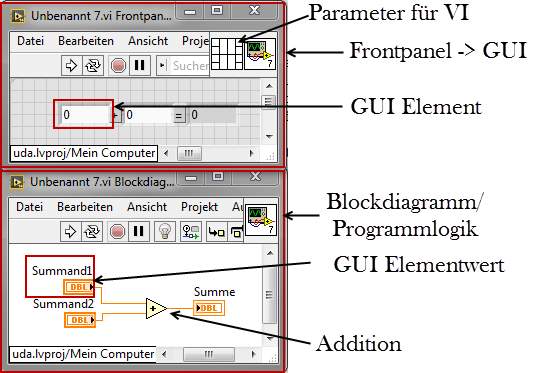
\includegraphics[width=0.6\textwidth]{pictures/LabVIEWExample}
		\caption{Beispiel LabView\gls{VI} mit Beschreibung}
		\label{fig:LabViewExample}
	\end{center}
\end{wrapfigure}
\gls{LabVIEW} ist eine grafische Programmiersprache, welche von National Instruments entwickelt wird. Die Funktionsweise von \gls{LabVIEW} ist zudem sehr speziell, da es Funktionsblöcke gibt, welche als Virtuelle Instrumente (\gls{VI}s) bezeichnet werden. Man kann sich die \gls{VI}s als Funktionen oder Methoden vorstellen. Sie besitzen immer ein \gls{Frontpanel} sowie ein \gls{Blockdiagramm}, in welchem auch der Code zu finden ist (Siehe Figure \ref{fig:LabViewExample}). Zudem unterstützt \gls{LabVIEW} seit geraumer Zeit Objektorientiertes Programmieren, dies jedoch nur sehr eingeschränkt verwendbar.
\newline
Die mangelnde Fähigkeit zur Objektorientierter Programmierung führt zu dem Umstand, dass an manchen Orten mit einer anderen Art und Weise angegangen werden muss, wie man es sich von Objektorientierten Programmieren gewohnt ist. Zudem sind \gls{LabVIEW} Programme nicht sonderlich schnell, weshalb besonders stark auf die Performance zu achten ist.
\newline
Eine weitere Sonderheit ist die Verknüpfung von GUIs mit dem Programm. Es besteht eine sehr starke Verknüpfung zwischen der Funktion und dem GUI. Dies bietet einige Vor- wie auch Nachteile. So wird in diesem Projekt stark mit \gls{Subpanel}s gearbeitet, welches die Möglichkeit liefert dynamisch GUIs von anderen\gls{VI}s in das laufende Programm einzubinden.  \footfullcite{website:labView} 


\subsection{Software}
\begin{wrapfigure}{l}{0.7\textwidth}
	\begin{center}
		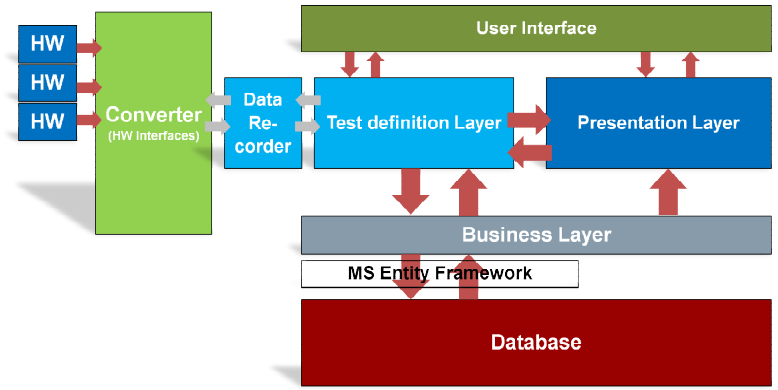
\includegraphics[width=0.65\textwidth]{pictures/SystemviewFTC}
		\caption{Systemview des Fire Test Commander}
		\label{fig:SystemViewFTC}
	\end{center}
\end{wrapfigure}
\subsubsection{Bestehende Software}
Im Rahmen des Umzuges der Testabteilung wurden die Brandräume neu gebaut. Während des Baus dieser Brandräume wurde zudem die veraltete Software, welche für die alten Brandräume erstellt wurde, durch eine Neue ersetzt. Die neu erstellte Software, welche unter dem Namen Fire Test Commander, fortan nur noch \acrshort{ftc} genannt, wurde mit \gls{LabVIEW} erstellt. Diese Software hat schon viele Ansätze, welche für die im Rahmen dieses Projektes zu implementierenden Programmes angewandt und übernommen werden können. Der \acrshort{ftc} bietet bereits eine Struktur um mit möglichst geringen aufwand Hardwarekomponenten hinzuzufügen (Siehe Figure \ref{fig:SystemViewFTC}). Diese Struktur, dient zudem gleich als Vorlage für die neu zu entwickelnde Software.
\newpage
\subsubsection{Systemgrenzen}
\begin{wrapfigure}{r}{0.4\textwidth}
	\begin{center}
		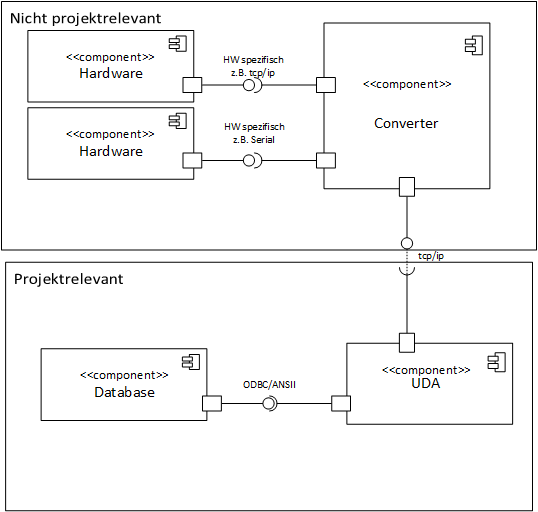
\includegraphics[width=0.35\textwidth]{pictures/Systemgrenzen}
		\caption{Systemabgrenzung der einzelnen Komponenten}
		\label{fig:SystemView}			
	\end{center}
\end{wrapfigure}
Da die Hardware Abstraktion komplett von der bestehenden Software übernommen werden kann, fällt diese aus dem Projekt heraus. Nur die UDA selber, soll als eigenständige Software entwickelt werden. Die Abgrenzung des Systemes kann in folgender Abbildung (Figure \ref{fig:SystemView}) nachvollzogen werden.
 Die Datenbank ist eine MySQL Datenbank, welche mithilfe des ODBC ANSII Treibers angesprochen werden kann. Die Schnittstelle wird von \gls{LabVIEW} zur Verfügung gestellt und musste auch nicht selber implementiert werden.
\subsubsection{Komponente UDA}
Aufgrund von Performance Gründen wurde die Software mit vielen verschiedenen Task ausgestattet. So ist jede GUI Komponente, welche auf dem Hauptprogramm aufrufbar ist, ein eigener Thread,  welcher seinen eigenen Event-Handler besitzt. Die GUI Komponenten werden zur entsprechenden Zeit dynamisch ins Hauptprogramm als Subpanels geladen. Diese komplexe Thread Struktur wird im Bild \ref{fig:LaufzeitansichtUDA} dargestellt.

Diese Software Struktur basiert auf dem Queued Message Handler Template von National Instruments.
Das Hauptprogramm (Main) besteht aus zwei parallelen Tasks:
\begin{itemize}
	\item dem Event-Handler, der primär auf Eingaben vom Anwender reagiert
	\item und der Verarbeitungstask (Queued Message Handler), der die Aufträge aus seiner Message-Queue entnimmt und der Reihe nach abarbeitet.
\end{itemize}

\begin{wrapfigure}{r}{0.4\textwidth}
	\begin{center}
		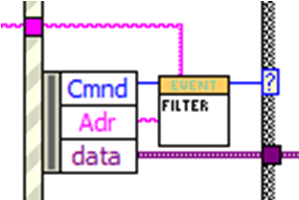
\includegraphics[width=0.3\textwidth]{pictures/filterVI}
		\caption{Aufruf des FilterVIs}
		\label{fig:filterVI}
	\end{center}
\end{wrapfigure}
Die Bedienoberfläche umfasst vier Subpanel-VIs. Diese werden im Hauptprogramm aufgerufen und laufen parallel zu den beiden Tasks des Hauptprogrammes. Das \gls{Frontpanel} eines dieser Subpanel-Vis wird programmatisch im Subpanel des Hauptprogrammes sichtbar gemacht.  
Jedes dieser Subpanel-Vis besitzt einen eigenen Event-Handler der auf Eingaben des Anwenders reagiert. Sowohl der Event-Handler des Hauptprogrammes wie auch diejenigen der Subpanel-Vis senden Messages an die Message-Queue der Verarbeitungstask im Hauptprogramm (In der Abbildung \ref{fig:LaufzeitansichtUDA} mit grünen durchgezogenen Pfeilen dargestellt).





\begin{wrapfigure}{l}{0.5\textwidth}
	\begin{center}
		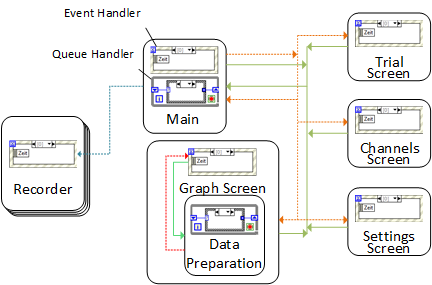
\includegraphics[width=0.5\textwidth]{pictures/LaufzeitansichtMitRecorder}
		\caption{Laufzeitansicht der GUI Tasks und deren Kommunikation}
		\label{fig:LaufzeitansichtUDA}
	\end{center}
\end{wrapfigure}
Die im Bild \ref{fig:LaufzeitansichtUDA} dargestellten Pfeile stellen die Kommunikationswege dar. Es gibt insgesammt 2 Möglichkeiten der Kommunikation. Wie oben geschrieben gibt es die Message-Queue, mit welcher Messages an das Hauptprogramm gesendet werden können. Dieses wiederum kann mit allen anderen über ein User-Event (In der Abbildung \ref{fig:LaufzeitansichtUDA} mit orangen gestrichelten Pfeilen dargestellt) kommunizieren. Die User-Events werden an alle Event-Handler gesendet (Broadcast). Mit Hilfe eines Filter-Vis (siehe Figure \ref{fig:filterVI}) kann der empfangende Event-Handler die Events aber filtern, sodass er nur Events mit der richtigen Adresse (ID) verarbeitet.  \footfullcite{tech:ftc} 

\begin{wrapfigure}{r}{0.4\textwidth}
	\begin{center}
		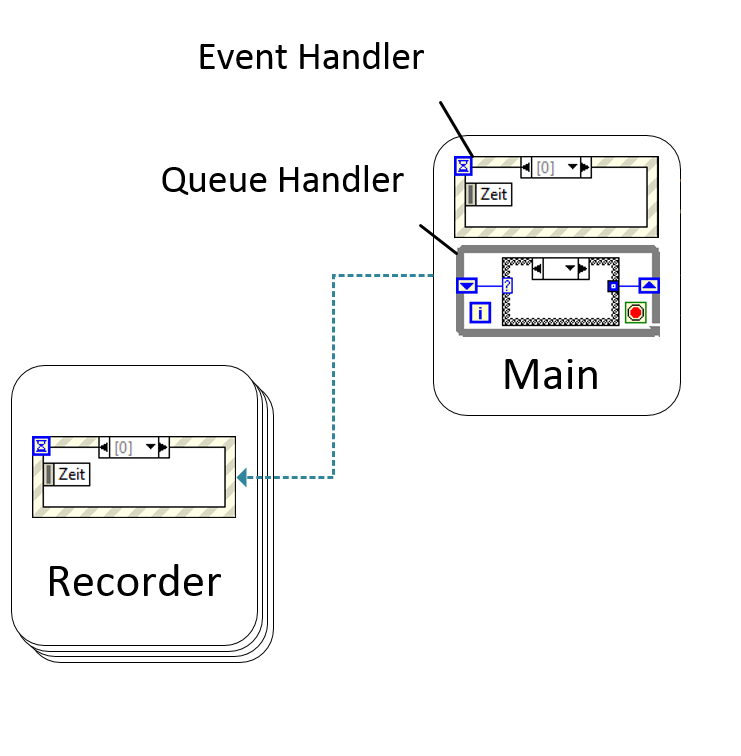
\includegraphics[width=0.29\textwidth]{pictures/LauftzeitansichtRecorderNah}
		\caption{Kommunikation Main mit Recorder}
		\label{fig:LauftzeitansichtRecorder}
	\end{center}
\end{wrapfigure}
\subsubsection{Data Preparation \& Recorder}
Die Umsetztung setzte voraus, dass das Aufzeichnen aller Daten in einem immer gleich bleibenden Intervall aufgezeichnet werden. Dazu war nötig, dass für jede angeschlossene Hardware ein eigener Thread startet, welcher die Daten zwischenspeichern kann. Um dies zu gewährleisten wurde ein Recorder-\gls{VI} erstellt, welcher über einen Asynchronen Aufruf mehrmals gestartet werden kann. Die Kommunikation zu diesen \gls{VI}s findet vom Hauptprogramm über einen Speziellen Event an alle laufenden Recorder statt(Siehe Figure \ref{fig:LauftzeitansichtRecorder}). Dieser Event wird jedoch an keinen der anderen Task gesendet. Der Event lässst schliesslich alle Recorder starten. Dieses Verhalten ist mit dem NotifyAll in Java vergleichbar, womit alle Thread zur selben Zeit gestartet werden können. 

\subsection{Datenbank}
\subsubsection{Bestehende Datenbank}
Mit der Implementierung der FTC Software wurde auch eine eigens dafür entwickelte Datenbank aufgebaut. Diese ist an sich enorm Komplex und sehr verstrickt, weshalb hier nicht viel näher auf diese eingegangen wird.
\subsubsection{Datenbank}
\begin{wrapfigure}{r}{0.480\textwidth}
	\begin{center}
		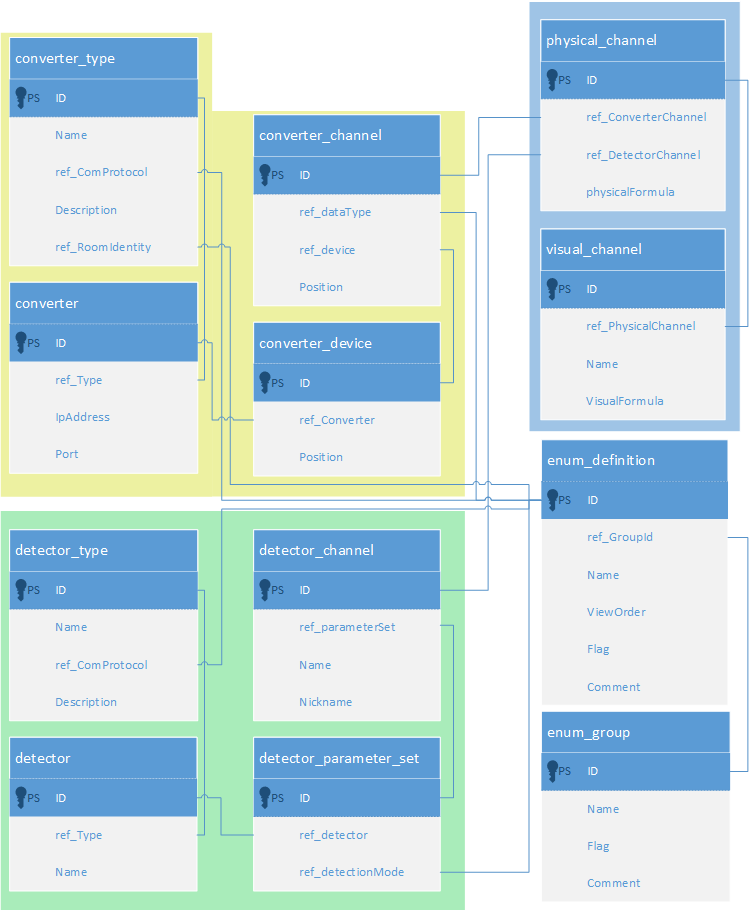
\includegraphics[width=0.44\textwidth]{pictures/DBShemaEasy2}
		\caption{Vereinfachtes DB-Schema für die UDA}
		\label{fig:DBSchemaUDA}
	\end{center}
\end{wrapfigure}

Da, wie schon erwähnt Software übernommen wird, so etwa die gesamte Hardwareabstraktion, muss auch die Datenbank an diesen Stellen übernommen werden. Um die Funktionalität der übernommenen Komponenten zu gewährleisten, wurde ein DB Schema der bisherigen Datenbank so abgespeckt (Siehe Figure \ref{fig:DBSchemaUDA}), dass sie für die UDA brauchbar ist.


Im Figure \ref{fig:DBSchemaUDA} wurden zusammengehörende Tabellen farblich zusammengelegt. Die Blau markierten Tabellen dienen dem einzelnen Versuch. So werden alle Visuellen Kanäle in der Visual Tabelle abgelegt. Hinter diesem sichtbaren Kanal liegt ein Physikalischer Kanal, welcher in der Physical Tabelle zu finden ist. An diesen Physikalischen Kanal sind die Meldeeinformationen, welche allesamt in der Grün markierten Fläche zu finden sind, angeschlossen, sowie die Hardware Kommunikationsinformationen, welche allesamt in der Gelb markierten Fläche zu finden sind, angeschlossen. In allem erhält man so einen Testaufbau, welcher dynamisch aus vordefinierten Geräten sowie Hardware Abstraktionen zusammengesetzt werden kann, in dem man die Blau markierten Tabellen verändert.
\section{Projektergebnis}
Es konnten die wesentliche Komponenten für die Aufzeichnung der Daten, sowie das Anzeigen jener Daten in einer neuen Datenerfassungssoftware erstellt werden. Diese Komponente werden in weiteren Schritten verbessert und erweitert. Die Software wurde schon nach den ersten erfolgreichen Datenaufzeichnungen verwendet und ist im Moment bei 2 Testaufbauten in Betrieb. Sie speichert die Daten persistent und erstellt auswertbare Excel Dateien, mit welchen die Testdesigner Auswertungen machen können.
Eine Installationsanleitung erleichtert zudem die Installation, da die Anleitung Schritt für Schritt mit Bildern erklärt wird. Die Softwaredokumentation sowie die Bedienungsanleitung wurden in Absprache mit den Vorgesetzten im Moment noch klein gehalten, da die Notwendigkeit einer funktionierenden Aufzeichnung die Dokumentation in den Hintergrund drängte. Der Grund für die unübliche Dringlichkeit, der Erstellung einer funktionierenden Aufzeichnungskomponente lag an einer Anpassung einer UL Norm, welche dafür sorgte, dass Melder mit einer neuen Apparatur, ohne vorhandene Datenerfassungssoftware, möglichst frühzeitig im Projekt getestet werden sollte.

\section{Arbeitsjournal}
\begin{center}
	\begin{tabular}{p{6cm} | l | r}
		\textbf{Tätigkeit} & \textbf{Zeitraum} & \textbf{Aufwand} \\ &&\textbf{(d a 8h)}\\
		\hline Analyse der Anforderungen & W1 & 1 \\
		\hline Einarbeitung in die Bestehende Software & W1 - W2 & 4 \\
		\hline Planung & W3 & 2.5 \\
		\hline SW-Design & W3-4 & 1.5 \\
		\hline DB-Modell & W4 & 1.5 \\
		\hline DB-Erstellen (Installieren und DB Modell umsetzten) & W4 - W5 & 1 \\
		\hline GUI Design & W5 & 2 \\
		\hline DB Kommunikation & W5 - W6 & 2.5 \\
		\hline Settings Screen (ini file Modifikation) & W6 - W7 & 2 \\
		\hline Channels Screen (Anzeige von DB Info) & W7 & 1.5 \\
		\hline Graph Screen (ohne Kommunikation) & W8 - W9 & 4 \\
		\hline Recorder Implementation (Kommunikation zu Hardware Komponenten) & W9 - W10 & 3.5 \\
		\hline Implementation Excel Export & W10 - W11 & 3 \\
		\hline Graph Screen Inbetriebnahme mit Kommunikation & W11 - W12 & 3 \\
		\hline Fertigstellung der Grundfunktionalität (Zusammenführen der Komponente) & W13 & 2 \\
		\hline Installer erstellen & W13 - W14 & 1 \\
		\hline Inbetriebnahme (Gebrauch der Software mit Ankunft des neuen Aufbaus) & W14 & 3 \\
		\hline Installationsanleitung & W14 & 1 \\
		\hline SW-Dokumentation (Beginn bei Planung wurde jeweils ergänzt und am Schluss nochmals zusammengetragen) & W14 & 0.5 \\\hhline{~--}
		& \textbf{Summe:} & \textbf{40.5} \\\hhline{~~=}
	\end{tabular}
\end{center}
\section{Fazit}
Für mich war und ist die UDA ein enorm grosses Projekt, welches mich sicher noch ein weiteres Jahr beschäftigen wird, da es noch viele Features zu implementieren gilt. Ich muss jedoch gestehen, dass ich die Arbeit unterschätzt habe. Es gab ja architektonisch schon eine Software von der ich Komponenten und Teile übernehmen konnte, so stellte mir \gls{LabVIEW} jedoch sehr viele Hindernisse in den Weg. Bei allen Objekten, welche ich von der bestehenden Software übernehmen wollte, musste ich viele Teile der Software neu implementieren, da \gls{LabVIEW} viele Probleme mit Abhängigkeiten bereitete. Weiter hatte ich einige Schwierigkeiten, bis ich das Aufzeichnen der Daten hingekriegt habe. Hier half jedoch, dass die Hardwarekomponenten schon klar eine Schnittstelle definiert hatten. Es dauerte jedoch sehr lange bis ich eine passende Lösung gefunden habe, da ich für die Integrität des Lesens, also dass die Software wirklich immer in einem gewissen Zeitintervall die Daten speichert, für jede Hardware Komponente einen eigenen Thread erstellen musste. Denn \gls{LabVIEW} weist hier auch so seine Eigenheiten auf, welche ich beachten musste. Als Fazit für mich muss ich leider sagen, dass ich persönlich im Moment für Projekte dieser Grössenordung von \gls{LabVIEW} abraten würde. Denn obwohl man schnell das Skelett des GUIs und eine gewisse Grundfunktionalität hat, lässt der Mangel an Wartbarkeit die Software Komplexität steigen. \gls{LabVIEW} unterstützt zwar inzwischen OOP und unit Tests, so sind diese jedoch im Moment noch nicht ausgereift und lassen die Verwendung teilweise nur eingeschränkt zu.
\section{Bestätigung Arbeitgeber}
\begin{center}
	\begin{tabular}{p{5.5cm} p{5.5cm}}
		\textbf{Auftraggeber} \\\hline
		Firma & Siemens Schweiz AG \\
		Name, Vorname & Schmid, Urs \\
		Funktion & Head of FireLab \\
		Strasse, Hausnummer & Gubelstrasse 22 \\
		PLZ, Ort & 6300, Zug \\
		Telefon & +41 79 503 9712 \\
		Email & urs.schmid@siemens.com \\
		&  \\
		\textbf{Verfasser} \\\hline
		Firma & Siemens Schweiz AG \\
		Name, Vorname & Wicki, Dane \\
		Funktion & Werkstudent(Informatik) \\
		Strasse, Hausnummer & Gubelstrasse 22 \\
		PLZ, Ort & 6300, Zug \\
		Telefon & +41 79 503 5181 \\
		Email & dane.wicki@siemens.com \\
		& \\
		& \\
		\multicolumn{1}{l|}{Urs Schmid, Auftraggeber}  & Dane Wicki, Verfasser  \\
		\multicolumn{1}{l|}{} &  \\
		\multicolumn{1}{l|}{} &  \\
		\multicolumn{1}{l|}{} &  \\\hhline{--}
	\end{tabular}
\end{center}
\printbibliography
\appendix
\printglossaries
\end{document}
